\chapter{Projektauftrag}

\label{AppendixProjektauftrag}

\section{Zweck des Dokuments}\label{ProjektauftragZweck}

Der Projektauftrag ist die verbindliche Vereinbarung zwischen Auftraggeber und
Projektleiter, und bildet die Grundlage für den Projektstart sowie die
Phasenfreigaben.

Folgend sind alle wichtigen Informationen die in der Phase Initialisierung
erarbeitet wurden. Alle weiteren Details die in der Initialisierung
ausgearbeitet wurden sind in der Studie im Anhang~\ref{AppendixStudie} zu
finden.

\section{Ausgangslage}\label{ausgangslage}

Als regelmässiger Konzertbesucher wünsche ich mir eine Plattform im
Internet, auf welcher ich eine zuverlässige Übersicht an Konzerten in
meiner Umgebung vorfinde. Heute sind die Events nur verteilt auf
verschiedenen Seiten wie die der Venues, des Konzertveranstalters, des
Künstlers oder auf Facebook publiziert.\\

\noindent
Ich möchte deshalb eine zentrale Plattform entwickeln, die es Benutzern
einfach macht, Konzerte für ihren Geschmack zu finden.
Die Plattform soll Genre unabhängig sein und entsprechende Filter anbieten.
Den Benutzern der Plattform soll es möglich sein, Konzerte selber zu
erfassen und pflegen.\\

\noindent
Um einen zusätzlichen Service für den Benutzer zur Verfügungs zu stellen,
ist es auch denkbar, eine Art Notifikationssystem zu bauen um Benutzer
über Handy-Notifications oder per Email an Konzerte oder Künstler zu
erinnern.\\

\noindent
Konzertveranstaltern kann das Erfassen ihrer Events vereinfacht werden,
indem auf der Plattform erfasste Veranstaltungen direkt auf den Sozialen
Medien wie Facebook, Twitter oder Instagram geteilt werden können.


\clearpage
\section{Projektziele}\label{projektziele}

Folgende Ziele sind in der Initialisierungsphase definiert worden:

\begin{longtable}[]{@{}lll@{}}
  \toprule
  Nr.  & Zielbeschreibung                                                                       & Muss/Kann\tabularnewline
  \toprule
       & Produktziele\tabularnewline
  \midrule
  1.1  & Besucher können im Produkt nach Konzerten suchen                                       & Muss\tabularnewline
  1.2  & Suchresultate können nach Musik-Genre und Ort gefiltert werden                         & Muss\tabularnewline
  1.3  & Das Produkt soll ein modernes responsives Design vorweisen                             & Muss\tabularnewline
  1.4  & Konzerte sollen von Suchmaschinen indexiert werden können                              & Muss\tabularnewline
  1.5  & Benutzer können isch im Produkt registrieren                                           & Muss\tabularnewline
  1.6  & Benutzer können ihr Passwort nach Verlust neu setzen                                   & Muss\tabularnewline
  1.7  & Inhalte des Portals sind durch die Benutzer erfassbar und bearbeitbar                  & Muss\tabularnewline
  1.8  & Kompatibilität mit aktuellem Google Chrome und Mozilla Firefox Browser                 & Muss\tabularnewline
  1.9  & Konzerte können vom Produkt nach Facebook exportiert werden                            & Kann\tabularnewline
  1.10 & Ein angemeldeter Benutzer kann vermerken ob er einem Konzert teilnimmt                 & Kann\tabularnewline
  1.11 & Das Produkt soll sich an Security Best-Practices von OWASP halten                      & Muss\tabularnewline
  \bottomrule
       & Abwicklungsziele\tabularnewline
  \midrule
  2.1  & \makecell[l]{Das Projekt soll nach HERMES 5 unter Berücksichtigung der Richtlinien von                            \\ der TSBE dokumentiert werden} & Muss\tabularnewline
  2.2  & Das Produkt muss bis Projektende fertiggestellt und bereit für die Einführung sein     & Muss\tabularnewline
  2.3  & Die Technische-Umsetzung wird durch Damian Senn erstellt                               & Muss\tabularnewline
  2.4  & \makecell[l]{Die Kommunikation zwischen Experten und Diplomanden erfolgt wie im                                   \\ Projektauftrag \ref{kommunikation} beschrieben.} & Muss\tabularnewline
  2.5  & Das Projekt muss bis Ende Mai 2019 abgeschlossen sein                                  & Muss\tabularnewline
  \bottomrule
\end{longtable}


\section{Rahmenbedingungen}\label{rahmenbedingungen}

\begin{itemize}
  \tightlist
  \item{}
    Das Projekt wird im Rahmen der Diplomarbeit durchgeführt.
  \item{}
    Die Richtlinien zum Erstellen des Diplomberichtes der TSBE.
    müssen eingehalten werden.
  \item{}
    Als Projektmethodik wird HERMES verwendet, angepasst auf das Projekt.
  \item{}
    Sämtliche Projekt-Dokumente sowie Programmcode wird regelmässig ins Github
    Repository\footnote{\url{https://github.com/topaxi/diplomarbeit-tsbe}} geladen.
\end{itemize}

% TODO: Do I need the following?
%\clearpage
%\subsection{Begründung der
%  Projektziele}\label{begruxfcndung-der-projektziele}

\clearpage
\section{Terminplan}\label{terminplan}

Nachfolgend ist der grobe Terminplan für die geplanten Phasen. Im Anhang~\ref{terminplan} ist
der detaillierte Terminplan abgelegt.

\begin{longtable}[]{@{}lrr@{}}
  \toprule
  Phase           & Datum                   & Stunden\tabularnewline
  \midrule
  \endhead
  Initialisierung & 06.03.2019 - 31.03.2019 & 64\tabularnewline
  Konzept         & 01.04.2019 - 21.04.2019 & 66\tabularnewline
  Realisierung    & 22.04.2019 - 19.05.2019 & 136\tabularnewline
  Abschluss       & 20.05.2019 - 26.05.2019 & 36\tabularnewline
  \midrule
                  & Total:                  & 286\tabularnewline
  \bottomrule
  \caption{Terminplan}
\end{longtable}


\section{Meilensteine}\label{meilensteine}

Im Projektplan wurden folgende Meilensteine und Termine festgelegt:

\begin{longtable}[]{@{}llcl@{}}
  \toprule
  Nr. & Meilenstein                     & KW & Datum\tabularnewline
  \midrule
  \endhead
  1   & Kickoff-Meeting                 & 10 & 06.03.2019\tabularnewline
  2   & Abschluss Phase Initialisierung & 13 & 31.03.2019\tabularnewline
  3   & Zwischen-Meeting                & 18 & 24.04.2019\tabularnewline
  4   & Abschluss Phase Konzept         & 16 & 21.04.2019\tabularnewline
  5   & Abschluss Phase Realisierung    & 20 & 19.05.2019\tabularnewline
  6   & Abschluss Phase Abschluss       & 21 & \tabularnewline
  7   & Abschluss-Meeting               & 22 & \tabularnewline
  \bottomrule
  \caption{Meilensteine}
\end{longtable}

Das Datum für das Abschluss-Meeting wird im Zwischen-Meeting mit den Experten, Sandro Bertolino und Severin Räz, festgelegt. Der Abschluss der Phase Abschluss ist Abhängig vom Abschluss-Meeting und wird mindestens eine Woche vor dem Meeting stattfinden.

\clearpage

\section{Organigramm}\label{organigramm}

\begin{figure}[!htb]
  \centering
  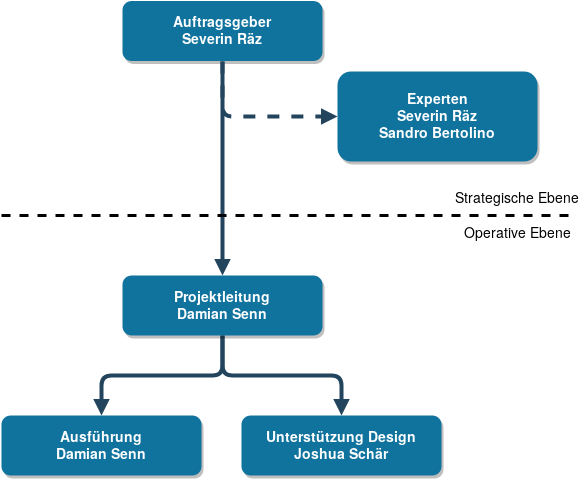
\includegraphics[width=0.8\textwidth]{figures/organigram.png}
  \caption{Organigram}
\end{figure}

\subsection{Tätigkeiten im Projekt}\label{tuxe4tigkeiten-im-projekt}

Für die Freigaben der Phasen ist nach Absprache mit Severin Räz Damian Senn
selbstständig verantwortlich.

\begin{longtable}[]{@{}ll@{}}
  \toprule
  \textbf{Name}    & \textbf{Funktions- und Tätigkeitsbereich}\tabularnewline
  \midrule
  \endhead
  Severin Räz      & Auftraggeber, externer Experte\tabularnewline
  Sandro Bertolino & Interner Experte\tabularnewline
  Damian Senn      & Projektleiter, Ausführung\tabularnewline
  Joshua Schär     & Unterstützung Design\tabularnewline
  \bottomrule
  \caption{Tätigkeiten Verteilung}
\end{longtable}

\subsection{Kommunikation}\label{kommunikation}

Wie im Kickoff-Meeting besprochen, wird Damian Senn alle zwei Wochen einen
kurzen Bericht an Sandro Bertolino und Severin Räz per E-Mail schicken.
Im Bericht wird erläutert was in der Zwischenzeit erledigt wurde und was
die nächsten Schritte im Projekt sind.

\clearpage

\section{Abgrenzungen}\label{abgrenzungen}

\begin{figure}[!htb]
  \centering
  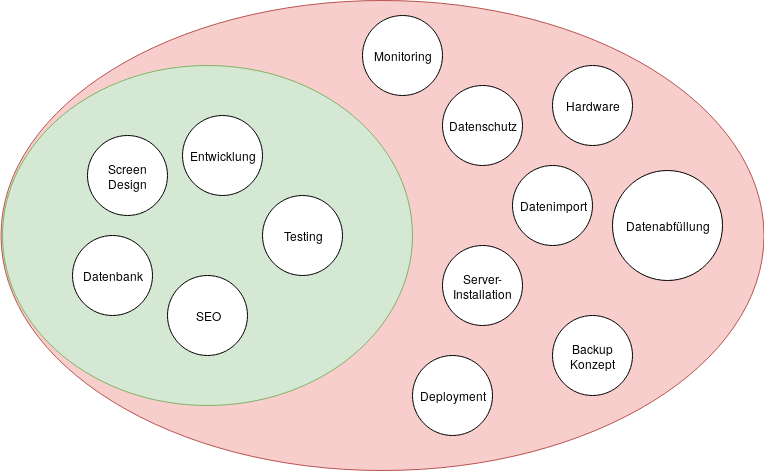
\includegraphics[width=0.95\textwidth]{figures/abgrenzungen.png}
  \caption{Abgrenzungen}
\end{figure}

\subsubsection{Hardware, Server-Installation, Deployment und
  Monitoring}\label{hardware-server-installation-deployment-und-monitoring}

Da das Projekt ein reines Software-Entwicklungs Projekt ist, werden
keine Operativen tätigkeiten wie Hardwarebeschaffung,
Server-Installation, Deployment und das einrichten eines
Monitoring-Systems vorgenommen.

\subsubsection{Datenschutz}\label{datenschutz}

Da das Projekt nicht deployed wird und somit nicht produktiv/online
gestellt wird, müssen im Rahmen dieser Projektarbeit noch keine Gedanken
über den Datenschutz gemacht werden.

\subsubsection{Datenimport}\label{datenimport}

Da wir bisher keine existierenden Konzertdaten besitzen, ist es nicht
nötig, einen Datenimport zu implementieren.

\subsubsection{Datenabfüllung}\label{datenabfuxfcllung}

Die Projektarbeit beinhaltet kein Datenset, Tests werden mit Testdaten
abgewickelt. Es liegt nicht in der Verantwortung des Projektleiters,
dass Daten in die Applikation abgefüllt werden.

\subsubsection{Backup Konzept}\label{backup-konzept}

Es wird kein Backup Konzept benötigt, da die Applikation im Rahmen
dieses Projektes nicht produktiv geschaltet wird.

\clearpage
\section{Anforderungskatalog}\label{anforderungskatalog}

Der Anforderungskatalog wurde in der Studie erarbeitet. Es wurden Kann und Muss
Kriterien definiert, wobei ein Muss-Kriterium zwingend erfüllt werden muss und
ein Kann-Kriterium als Erweiterung angesehen wird.

% TODO: Fix multirows across pages
%       https://tex.stackexchange.com/questions/79143/how-to-repeat-cell-content-on-next-page-for-longtable-using-multirow/79152
\begin{longtable}[]{@{}p{1.9cm}p{2.5cm}cp{5.5cm}cc@{}}
  \toprule
  \textbf{Feature}           & \textbf{Titel}             & \textbf{Nr.} & \textbf{Kriterium}                                                                                          & \textbf{Ziel} & \textbf{Muss}\tabularnewline
  \midrule
  \endhead
  \multirow{10}{*}{Suche}    & Suche nach Konzertname     & 1.1          & Listet alle Konzerte die Wörter der Suche im Konzertnamen beinhalten                                        & 1.1           & \textbf{Muss}                \\ \cline{2-6}
                             & Suche nach Konzertlocation & 1.2          & Schränkt die Such-Resultate nach gegebener Konzertlocation ein                                              & 1.2           & \textbf{Muss}                \\ \cline{2-6}
                             & Suche nach Ort             & 1.2          & Schränkt die Such-Resultate nach gegebenem Ort ein                                                          & 1.2           & \textbf{Muss}                \\ \cline{2-6}
                             & Suche nach Genre           & 1.2          & Schränkt die Such-Resultate nach gegebenem Musik-Genre ein                                                  & 1.2           & \textbf{Muss}                \\
  \midrule
  \multirow{8}{*}{Design}    & Desktop                    & 2.1          & Alle Ansichten haben eine Desktop-Optimierte Variante                                                       & 1.4           & \textbf{Muss}                \\ \cline{2-6}
                             & Tablet                     & 2.2          & Alle Ansichten haben eine Tablet-Optimierte Variante                                                        & 1.4           & \textbf{Muss}                \\ \cline{2-6}
                             & Mobile                     & 2.3          & Alle Ansichten haben eine Mobile-Optimierte Variante                                                        & 1.4           & \textbf{Muss}                \\ \cline{2-6}
                             & Browser Kompatibilität     & 2.4          & Alle Ansichten müssen in aktuellem Google Chrome und Mozilla Firefox dem Grundlayout folgen                 & 1.9           & \textbf{Muss}                \\
  \midrule
  \multirow{4}{*}{SEO}       & Indexierbarkeit            & 3.1          & Das Produkt ist von Suchmaschinen indexierbar                                                               & 1.5           & \textbf{Muss}                \\ \cline{2-6}
                             & Linked Data                & 3.2          & Konzert Detailseiten sind mit dem Event-Schema\footnote{\url{https://schema.org/Event}} ausgestattet              & 1.5           & \textbf{Muss}                \\
  \midrule
  \multirow{8}{*}{Benutzer}  & Registrierung              & 4.1          & Besucher können sich einen Benutzer registrieren, Benutzernamen und E-Mail Adressen müssen einzigartig sein & 1.6           & \textbf{Muss}                \\ \cline{2-6}
                             & Passwort-Vergessen         & 4.2          & Benutzer können sich einen Passwort-Reset Link anfordern                                                    & 1.7           & \textbf{Muss}                \\ \cline{2-6}
                             & Social                     & 4.3          & Benutzer können auf Konzerten vermerken ob sie Teilnehmen oder nicht                                        & 1.11          & Kann                         \\
  \midrule
  \clearpage
  \multirow{6}{*}{Erfassung} & Artist                     & 5.1          & Benutzer können Artisten mit einem Genre erfassen                                                           & 1.8           & \textbf{Muss}                \\ \cline{2-6}
                             & Location                   & 5.2          & Benutzer können eine Konzertlocation mit Ort/Strasse erfassen                                               & 1.8           & \textbf{Muss}                \\ \cline{2-6}
                             & Konzert                    & 5.3          & Benutzer können ein Konzert mit Konzertlocation und Artisten erfassen                                       & 1.8           & \textbf{Muss}                \\ \cline{2-6}
                             & Facebook                   & 5.4          & Benutzer können ein Konzert in ein Facebook-Event exportieren                                               & 1.10          & Kann                         \\
  \midrule
  \multirow{9}{*}{Security}  & SQL-Injection              & 6.1          & Das Produkt soll resistent gegen SQL-Injection sein                                                         & 1.12          & \textbf{Muss}                \\ \cline{2-6}
                             & HTML-Injection             & 6.2          & Das Produkt soll resistent gegen HTML-Injection / XSS sein                                                  & 1.12          & \textbf{Muss}                \\ \cline{2-6}
                             & Passwort encryption        & 6.3          & Passwörter von Benutzer müssen mit einem sicheren Verfahren gespeichert werden                              & 1.12          & \textbf{Muss}                \\ \cline{2-6}
                             & Session                    & 6.4          & Session-Cookies dürfen nicht durch JavaScript ausgelesen werden                                             & 1.12          & Kann                         \\
  \midrule
  Performance                & Ladezeit                   & 7.1          & Die Seitenansichten dürfen nicht länger als 6 Sekunden auf einem 3G Netz laden                              &               & \textbf{Muss}                \\
  \midrule
  Sonstiges                  & User Tracking              & 8.1          & Benutzerverhalten soll analysiert und nachvollziehbar sein.                                                 &               & Kann                         \\
  \bottomrule
  \caption{Anforderungskatalog}
\end{longtable}


\clearpage
\section{Lösungsbeschreibung}\label{loesungsbeschreibung}

In der Studie (Anhang~\ref{AppendixStudie}) wurden Technologien gegenüber
gestellt und für die Umsetzung mittels Nutzwertanalysen ausgewählt.\\

\noindent
Folgende Technologien wurden ausgewählt:\\

\textbf{Browser sowie Server Technologie:}

\begin{figure}[!htb]
  \centering
  
\includegraphics[width=0.8\textwidth]{figures/phoenix.png}
  \captionsource{Phoenix Framework Logo}{\url{https://github.com/phoenixframework/phoenix}}
\end{figure}

\noindent
Die Nutzerwertanalyse hat ergeben, dass es sinnvoller ist, das Projekt mit
einer klassischen SSR Applikation zu starten. Das Phoenix Framework bietet alle
benötigten Features an und kann durch Module einfach erweitert werden.

Für dynamische Interaktionen wie Formular-Validierungen wird zu einfachem
JavaScript gegriffen. Ist ein Screen besonders interaktiv, kann gegebenenfalls
eine kleinere JavaScript-Library verwendet werden um die Problemlösung zu
vereinfachen.\\

\textbf{Testing Technologie:}

\begin{figure}[!htb]
  \centering
  
\includegraphics[width=0.8\textwidth]{figures/wallaby.png}
  \captionsource{Wallaby Logo}{\url{https://github.com/keathley/wallaby}}
\end{figure}

\noindent
Getestet wird die Applikation durch die von Phoenix gegebenen Testing-Tools
sowie mit der Browser-Testing Library «Wallaby».

\clearpage
\section{Kosten}\label{projektauftragkosten}

In der Studie wurden die Projekt- sowie Betriebskosten ausgerechnet.

Der gesamte Personalaufwand beträgt \textbf{42'900} für die geplanten Stunden.

\begin{longtable}[]{@{}lrr@{}}
  \toprule
  \textbf{Phase}  & \makecell[r]{\textbf{Geplante} \\\textbf{Stunden}} & \textbf{Kosten}\tabularnewline
  \midrule
  \endhead
  Initialisierung &  64                       &  9'600.- CHF\tabularnewline
  Konzept         &  66                       &  9'900.- CHF\tabularnewline
  Realisierung    & 136                       & 20'400.- CHF\tabularnewline
  Abschluss       &  64                       &  5'400.- CHF\tabularnewline
  \midrule
  \textbf{Total:} & 286                       & 42'900.- CHF\tabularnewline
  \bottomrule
  \caption{Projektkosten}
\end{longtable}


Für die Betriebskosten wurde angenommen, dass das Produkt in der Cloud auf
einer mittelgrossen Umgebung betrieben wird. Die Kosten dieser Umgebung wurde
auf 150.- CHF pro Monat geschätzt.

Neben der Umgebung muss mindestens eine Domain gekauft und jährlich bezahlt
werden. Die Kosten einer Domain sind rund 20.- CHF pro Jahr.

Da jediglich Open Source Software eingesetzt wird, gibt es keine
Software-Lizenzen zu bezahlen.

\begin{longtable}[]{@{}lll@{}}
  \toprule
  \textbf{Kostenstelle} & \textbf{Jährliche Kosten}\tabularnewline
  \midrule
  \endhead
  Software              & Keine\tabularnewline
  .com Domain           & 20.- CHF\tabularnewline
  Hosting               & 1'800.- CHF\tabularnewline
  \midrule
  \textbf{Total:}       & 1'820.- CHF\tabularnewline
  \bottomrule
  \caption{Betriebskosten}
\end{longtable}


\clearpage
\section{Risiken}\label{risiken}

Die Risikobewertung erfolgt mit folgender Formel:\\

\textbf{Bewertung = Schaden x Eintrittswahrscheinlichkeit}\\

\noindent
Schadensskala:

\begin{longtable}[]{@{}lp{11cm}@{}}
  \toprule
  \textbf{Gewichtung} & \textbf{Beschreibung}\tabularnewline
  \midrule
  \endhead
  Gering (1-2)        & Kleiner Schaden, hat kaum Auswirkungen auf das Projekt.\tabularnewline
  Mittel (3-4)        & Mittlerer Schaden, Zeitverzögerungen oder Qualitätsverluste.\tabularnewline
  Hoch (5-6)          & Hoher Schaden, wichtige Arbeiten oder Phasen können nicht abgeschlossen werden, schlimmstenfalls ein Abbruch des Projekts.\tabularnewline
  \bottomrule
  \caption{Risiken - Schadensskala}
\end{longtable}

\noindent
Eintrittswahrscheinlichkeitsskala:

\begin{longtable}[]{@{}lp{12cm}@{}}
  \toprule
  \textbf{Gewichtung} & \textbf{Beschreibung}\tabularnewline
  \midrule
  \endhead
  Gering (1-2)        & Kleine Eintrittswahrscheinlichkeit.\tabularnewline
  Mittel (3-4)        & Mittlere Eintrittswahrscheinlichkeit.\tabularnewline
  Hoch (5-6)          & Hohe Eintrittswahrscheinlichkeit.\tabularnewline
  \bottomrule
  \caption{Risiken - Eintrittswahrscheinlichkeit}
\end{longtable}

\noindent
Handlungen um Risikobewertungen zu senken:

\begin{longtable}[]{@{}lp{12cm}@{}}
  \toprule
  \textbf{Handlung} & \textbf{Beschreibung}\tabularnewline
  \midrule
  \endhead
  Akzeptanz         & Das Eintreten eines Risiko wird wissentlich angenommen.\tabularnewline
  Transfer          & Die Verantwortung von Risiken können an Dritte abgegeben werden.\tabularnewline
  Verminderung      & Der Schaden oder die Eintrittswahrscheinlichkeit kann begrenzt oder reduziert werden.\tabularnewline
  Vermeidung        & Es kann jeglichen Schaden vermieden werden.\tabularnewline
  \bottomrule
  \caption{Risiken - Handlungen zur Senkung der Bewertung}
\end{longtable}


\clearpage
\subsection{Projektrisiken}\label{projektrisiken}

\begin{longtable}[]{@{}lp{3cm}p{4cm}ccc@{}}
  \toprule
  \textbf{Nr.} & \textbf{Risiko}                             & \textbf{Auswirkung}                                 & \textbf{Schaden} & \textbf{Wahrsch.} & \textbf{Bewertung}\tabularnewline
  \midrule
  \endhead
  1            & Ausfall des Entwicklers oder Projektleiters & Verzögerungen von Arbeiten                          & 4                & 3                 & Mittel\tabularnewline
  2            & Unvollständige Projektdokumentation         & Schlechtere Diplomarbeit Bewertung                  & 4                & 2                 & Mittel\tabularnewline
  3            & Schlechter Projektplan                      & Verzögerungen und eventuelle Qualitätsverluste      & 4                & 3                 & Mittel\tabularnewline
  4            & Keine Benutzer                              & Das Produkt wird nicht von Benutzern eingesetzt     & 3                & 4                 & Mittel\tabularnewline
  5            & Technisch nicht umsetzbare Features         & Das Produkt kann nicht wie angedacht benutzt werden & 4                & 3                 & Mittel\tabularnewline
  \bottomrule
  \caption{Projektrisiken}
\end{longtable}

\clearpage
\subsection{Massnahmen}\label{massnahmen}

\begin{longtable}[]{@{}lp{4.1cm}lccc@{}}
  \toprule
               &                                                                       &                   & \multicolumn{3}{l}{\textbf{Bewertung nach Massnahme}}\tabularnewline
  \textbf{Nr.} & \textbf{Massnahme}                                                    & \textbf{Handlung} & \textbf{Schaden}                                                     & \textbf{Wahrsch.} & \textbf{Bewertung}\tabularnewline
  \midrule
  \endhead
  1            & Arzt aufsuchen, ggf. Projekt-Pause oder Abbruch                       & Akzeptanz         & 4                                                                    & 3                 & Mittel\tabularnewline
  2            & Statusbericht alle zwei Wochen, bei Fragen sofort Hilfe suchen        & Verminderung      & 2                                                                    & 1                 & Gering\tabularnewline
  3            & Genügend Buffer-Zeit einplanen, ggf. Ferientage für Projekt einsetzen & Verminderung      & 2                                                                    & 1                 & Gering\tabularnewline
  4            & Das Produkt löst vor allem ein persönliches Interesse                 & Akzeptanz         & 3                                                                    & 4                 & Mittel\tabularnewline
  5            & Vereinfachte Alternativen in Konzept-Phase untersuchen                & Verminderung      & 2                                                                    & 2                 & Gering\tabularnewline
  \bottomrule
  \caption{Projektrisiken - Massnahmen}
\end{longtable}

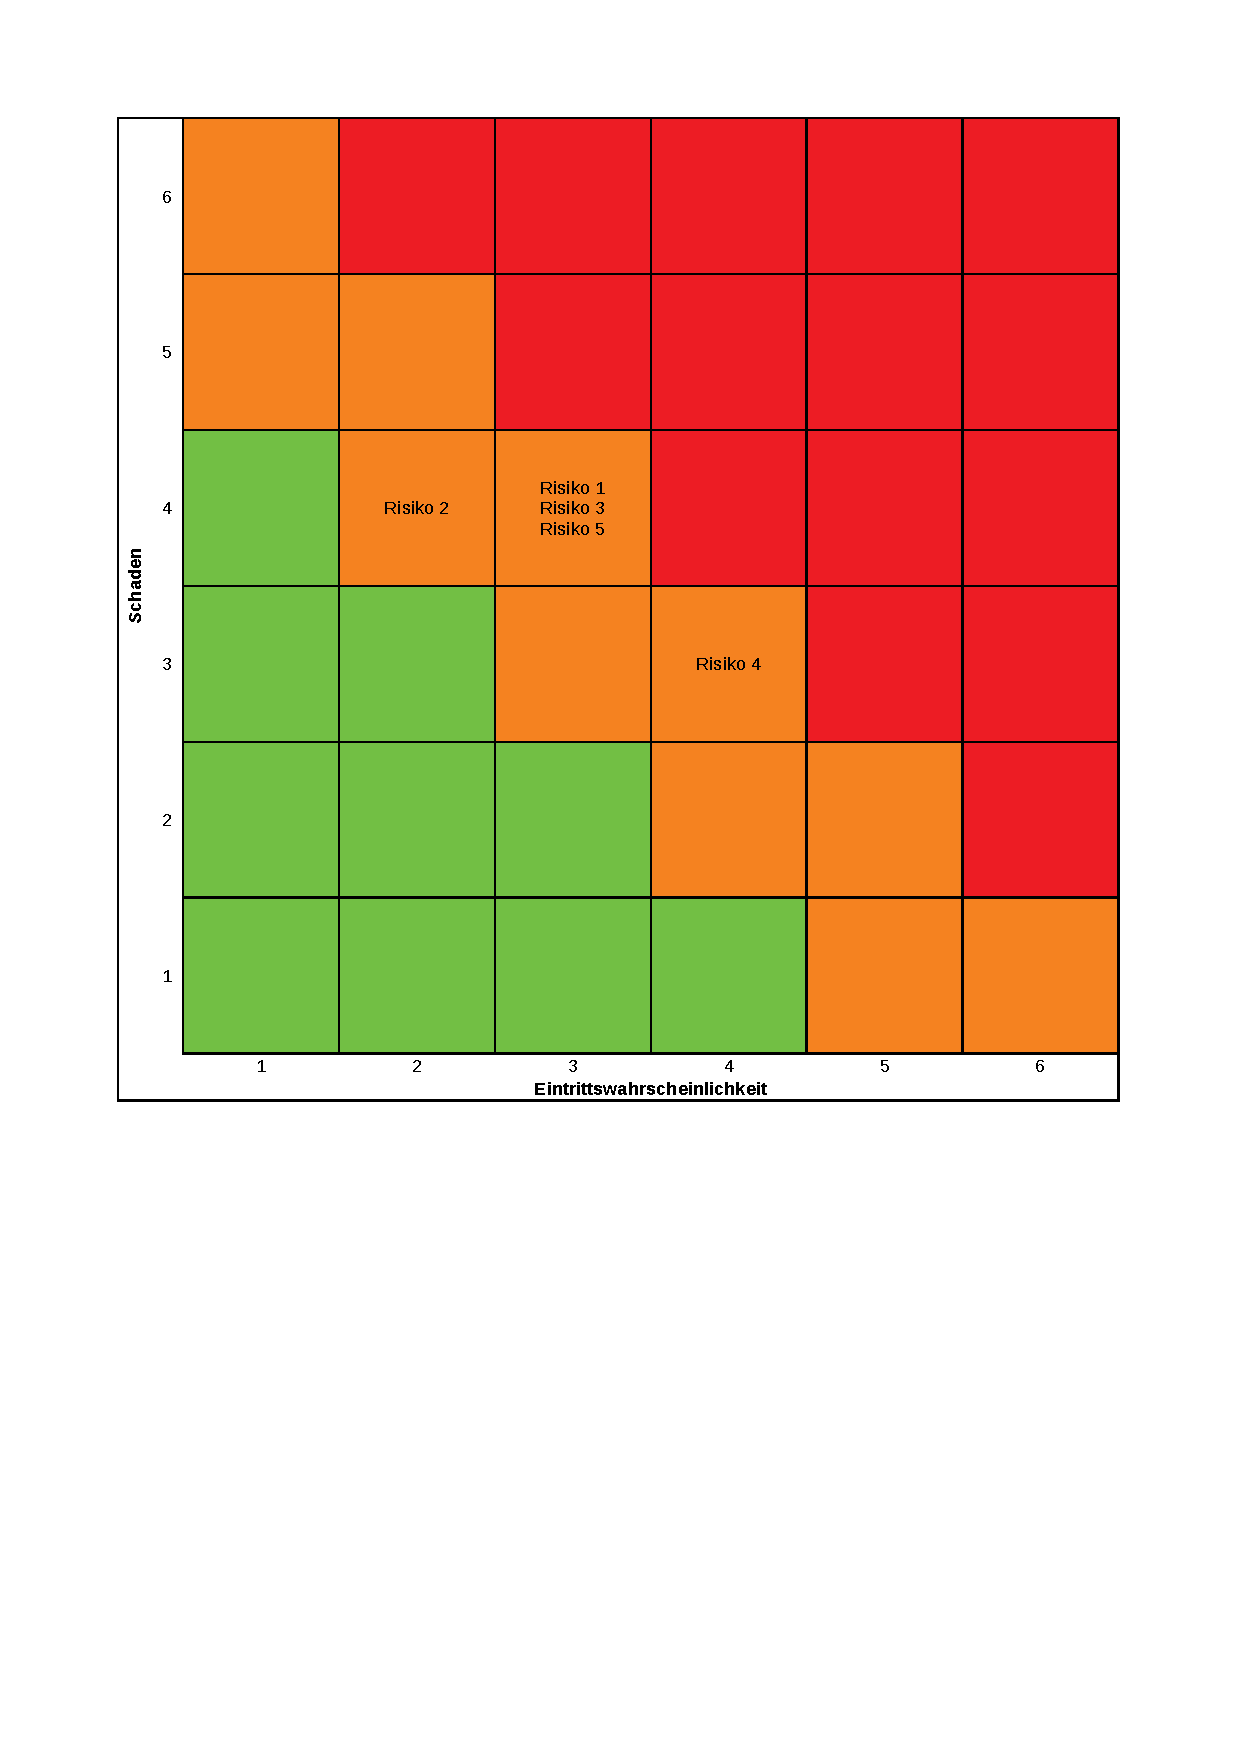
\includepdf[pages=1, pagecommand={\subsection{Risikodiagramm ohne Massnahmen}\label{risikodiagram-ohne-massnahmen}}, trim=0mm 80mm 0mm 0mm, clip]{initialisierung/risiko.pdf}
\includepdf[pages=2, pagecommand={\subsection{Risikodiagramm mit Massnahmen}\label{risikodiagram-mit-massnahmen}}, trim=0mm 80mm 0mm 0mm, clip]{initialisierung/risiko.pdf}
